\section{Experiments}\label{s:exp}
\paragraph{Datasets.} 
We conduct the experiments on the most widely used machine translation benchmarks: WMT14 English-German~(WMT14 EN-DE, 4.5M pairs)\footnote{\url{https://drive.google.com/uc?export=download&id=0B_bZck-ksdkpM25jRUN2X2UxMm8}} and IWSLT14 German-English~(IWSLT14, 160K pairs)\footnote{ \url{https://github.com/pytorch/fairseq}}. 
The datasets are processed with the Moses script~\citep{Moses}, and the words are segmented into subword units using byte-pair encoding~\citep[BPE]{bpe}.  
We use the shared subword embeddings between the source language and target language for the WMT datasets and the separated subword embeddings for the IWSLT14 dataset.
   
\paragraph{Model Setting.} 
In the case of IWSLT14 task, we use a small setting~($d_\text{model}$ = 256, $d_\text{hidden}$ = 512, $p_\text{dropout}$ = 0.1, $n_\text{layer}$ = 5 and $n_\text{head}$ = 4) for Transformer and NAT models. 
For the WMT tasks, we use the \texttt{Transformer-base} setting~($d_\text{model}$ = 512, $d_\text{hidden}$ = 512, $p_\text{dropout}$ = 0.3, $n_\text{head}$ = 8 and $n_\text{layer}$ = 6) of the~\citet{transformer}. 
We set the hyperparameter $\alpha$ used in Eq.~\ref{eqn:loss} and $\lambda$ in Eq.~\ref{eqn:ema_c}-\ref{eqn:ema_q} to 1.0 and 0.999, respectively.
The categorical number $K$ is set to 64 in our experiments.
We implement our model based on the open-source framework of \texttt{fairseq}~\cite{fairseq}.

\paragraph{Optimization.} 
We optimize the parameter with the Adam~\citep{adam} with $\beta=(0.9,0.98)$. 
We use inverse square root learning rate scheduling~\citep{transformer} for the WMT tasks and linear annealing schedule~\cite{iter_nat} from $3\times10^{-4}$ to $1\times10^{-5}$ for the IWSLT14 task.
Each mini-batch consists of 2048 tokens for IWSLT14 and 32K tokens for WMT tasks.

\paragraph{Distillation.}
Sequence-level knowledge distillation~\citep{hinton2015distilling} is applied to alleviate the multi-modality problem~\cite{nat} while training. 
We follow previous studies on NAT~\citep{nat,iter_nat,imitate_nat} and use translations produced by a pre-trained autoregressive Transformer~\cite{transformer} as the training data.
% , which significantly improves the performance. 
% We follow this setting and use our pretrained Transformer as the teacher to distill the training data.

\paragraph{Reranking.}
We also include the results that come at reranked parallel decoding~\citep{nat,enat,nat_reg,imitate_nat}, which generates several decoding candidates in parallel and selects the best via re-scoring using a pre-trained autoregressive model. 
Specifically, we first predict the target length $\hat{m}$ and generate output sequence with $\arg\max$ decoding for each length candidate $m \in [\hat{m}-\Delta m, \hat{m}+\Delta m ]$~($\Delta m$ = 4 in our experiments, means there are $N=9$ candidates), which was called length parallel decoding~(LPD). 
Then, we use the pre-trained teacher to rank these sequences and identify the best overall output as the final output.

\paragraph{Baselines.}
We compare the \method with several strong NAT baselines, including:
\begin{itemize}
    \item The NAT builds upon latent variables: NAT-FT~\cite{nat}, LT~\cite{lt}, Syn-ST~\cite{syn_st}, LV-NAR~\cite{lv_nar} and Flowseq~\cite{flowseq}.
    \item The NAT with extra autoregressive decoding or iterative refinement: NAT-DCRF~\cite{nat_crf}, IR-NAT~\cite{iter_nat}, and CMLM~\cite{cmlm}.
    \item The NAT with auxiliary training objectives: NAT-REG~\cite{nat_reg}, imitate-NAT~\cite{imitate_nat}.
\end{itemize}
% For the sake of fairness, we choose the \texttt{Transformer-base} setting for all baselinses. 
We compare the proposed \method against baselines both in terms of generating quality and inference speedup. 
For all our tasks, we obtain the performance of baselines by either directly using the performance figures reported in the previous works if they are available or producing them by using the open-source implementation of baseline algorithms on our datasets. 

\paragraph{Metrics.}
We evaluate using the tokenized and cased BLEU scores~\citep{bleu}. 
We highlight the best \textbf{NAT result} with bold text.

\subsection{Results}

\begin{table}[tbp]
\centering
\small
\begin{tabular}{lccc}
\toprule
\multirow{2}{*}{Model} & \multicolumn{2}{c}{WMT14} & IWSLT14\\
                       & EN-DE       & DE-EN     & DE-EN \\
\midrule
LV-NAR                 & 11.80       & /         & / \\
% CMLM                   & 10.88       & /          \\ 
% Flowseq                & 18.55       & 23.36      \\
AXE CMLM               & 20.40       & 24.90     & / \\
SynST                  & 20.74       & 25.50     & 23.82\\  
Flowseq                & 20.85       & 25.40     & 24.75\\
\midrule
NAT~(ours)             & 9.80        & 11.02     & 17.77\\
\method~(ours)         & \textbf{21.30} & \textbf{25.73} & \textbf{29.81}\\
\bottomrule
\end{tabular}
\caption{Results of the NAT models with argmax decoding on test set of WMT14 and IWSLT14.}
\label{tab:pure_mt}
\end{table}

\paragraph{Translation Quality.}
First, we compare~\method with the NAT models without using advanced techniques, such as knowledge distillation, reranking, or iterative refinements.
The results are listed in Table~\ref{tab:pure_mt}.
The \method achieves significant improvements~(around 11.5 BLEU in EN-DE, more than 14.5 BLEU in DE-EN) over the vanilla NAT, which indicates that modeling categorical information could improve the modeling capability of the NAT model. 
Also, the \method achieves better results than Flowseq and SynST, which demonstrates the effectiveness of \method in modeling dependencies between the target outputs.

\begin{table}[tbp]
\centering
\small
\begin{tabular}{lccc}
\toprule
\multirow{2}{*}{Model}  & \multicolumn{2}{c}{WMT14} & IWSLT14 \\
                        & EN-DE         & DE-EN     & DE-EN \\
\midrule
NAT-FT                  & 17.69         & 21.47     &   /   \\
LT                      & 19.80         & /         &   /   \\
% IR-NAR             & 13.91       & 16.77      \\
% CMLM                 & 15.06       & 19.26      \\
% ENAT                 & 20.65       & 23.02      \\
NAT-REG                 & 20.65         & 24.77     & 23.89 \\
imitate-NAT             & 22.44         & 25.67     &   /   \\
% Flowseq            & 21.45       & 26.16      \\
Flowseq                 & 23.72         & 28.39     & 27.55 \\
NAT-DCRF                &  23.44        & 27.22     & 27.44 \\
% CMLM-base              & 18.05       & 21.83      \\
\midrule
Transformer~(ours)      & 27.33         & 31.69     & 34.29 \\
NAT~(ours)              & 17.69         & 18.93     & 23.78 \\
\method~(ours)          & \textbf{25.56}&\textbf{29.36} & \textbf{31.15}  \\
\bottomrule
\end{tabular}
\caption{Results of NAT models trained with knowledge distillation on test set of WMT14 and IWSLT14.}
\label{tab:kd_mt}
\end{table}

The performance of the NAT models with advance techniques~(sequence-level knowledge distillation or reranking) is listed in Table~\ref{tab:kd_mt} and Table~\ref{tab:lpd_mt}.
Coupling with the knowledge distillation techniques, all NAT models achieve remarkable improvements.

\begin{table}[tbp]
\centering
\small
\begin{tabular}{lccc}
\toprule
\multirow{2}{*}{Model}  & \multirow{2}{*}{N} & \multicolumn{2}{c}{WMT14} \\
                        &                    & EN-DE       & DE-EN      \\
\midrule
% \multirow{2}{*}{NAT-FT} & 10                 & 18.66       & 22.42      \\
%                       & 10                 & 18.66       & 22.42      \\
%\midrule
NAT-FT                  & 10                 & 18.66       & 22.42      \\
NAT-FT                  & 100                & 19.17       & 23.20      \\
LT                      & 10                 & 21.00       & /          \\
LT                      & 100                & 22.50       & /          \\
% ENAT                  & 9                  & 24.28       & 26.10      \\
NAT-REG                 & 9                  & 24.61       & 28.90      \\
imitate-NAT             & 9                  & 24.15       & 27.28      \\
% Flowseq               & 30                 & 23.48       & 28.40      \\
Flowseq                 & 15                 & 24.70       & 29.44      \\
Flowseq                 & 30                 & 25.31       & 30.68      \\
NAT-DCRF                & 9                  & 26.07       & 29.68      \\
NAT-DCRF                & 19                 & \textbf{26.80}       & 30.04      \\
\midrule
Transformer (ours)      & -                  & 27.33       & 31.69      \\
\method (ours)          & 9                  & 26.60       & \textbf{30.75}     \\
\bottomrule 
\end{tabular}
\caption{Results of NAT models with parallel decoding on test set of WMT14. ``N'' means the number of candidates to be re-ranked.}
\label{tab:lpd_mt}
\end{table}

Our best results are obtained with length parallel decoding, which employs a pretrained Transformer to rerank the multiple parallels generated candidates of different target lengths.
Specifically, on a large scale WMT14 dataset, \method surpasses the NAT-DCRF by 0.71 BLEU score in DE-EN but slightly under the NAT-DCRF around 0.20 BLEU in EN-DE, which shows that the~\method is comparable to the state-of-the-art NAT model.
Also, we can see that a larger ``N'' leads to better results~($N=100$ vs. $N=10$ of NAT-FT, $N=19$ vs. $N=9$ of NAT-DCRF, etc.); however, it always comes at the degradation of decoding efficiency.

\begin{table}[tbp]
\centering
\tabcolsep 4pt
\small
\begin{tabular}{lcccc}
\toprule
\multirow{2}{*}{Model}      & \multirow{2}{*}{Iteration} & \multicolumn{3}{c}{WMT14} \\
                            &                            & EN-DE         & DE-EN     & Speedup\\
\midrule
\multirow{4}{*}{IR-NAT}     & 1                          & 13.91         & 16.77     & 11.39$\times$ \\
                            & 2                          & 16.95         & 20.39     & 8.77$\times$\\
                            & 5                          & 20.26         & 23.86     & 3.11$\times$\\
                            & 10                         & 21.61         & 25.48     & 2.01$\times$\\
\midrule
% \multirow{3}{*}{CMLM-small} & 1                          & 15.06         & 19.26      \\
%                             & 4                          & 24.17         & 28.55      \\
%                             & 10                         & 25.51         & 29.47      \\
% \midrule
\multirow{2}{*}{CMLM}  & 4                          & 26.08         & 30.11     &  / \\
                            & 10                         & \textbf{26.92}& \textbf{30.86}&  /   \\
\midrule
\method              & 1                          & 25.56         & 29.36        & 10.37$\times$ \\
\method (N=9)         & 1                          & 26.60         & 30.75        & 5.59$\times$ \\
\bottomrule
\end{tabular}
\caption{Results of NAT models with iterative refinements on test set of WMT14. ``Iteration'' means the number of iteration refinements.}
\label{tab:iter_mt}
\end{table}

We also compare our \method with the NAT models that employ an iterative decoding technique and list the results in Table~\ref{tab:iter_mt}.
The iterative-based non-autoregressive Transformer captures the target language's dependencies by iterative generating based on the previous iteration output, which is an important exploration for a non-autoregressive generation. 
With the iteration number increasing, the performance improving, the decoding speed-up dropping,  whatever the IR-NAT or CMLM.
We can see that the \method achieves a better result than the CMLM with four iterations and IR-NAT with ten iterations, even close to the CMLM with ten iterations while keeping the benefits of a one-shot generation. 

\begin{figure*}[tbp]
    \begin{subfigure}[t]{0.495\linewidth}
    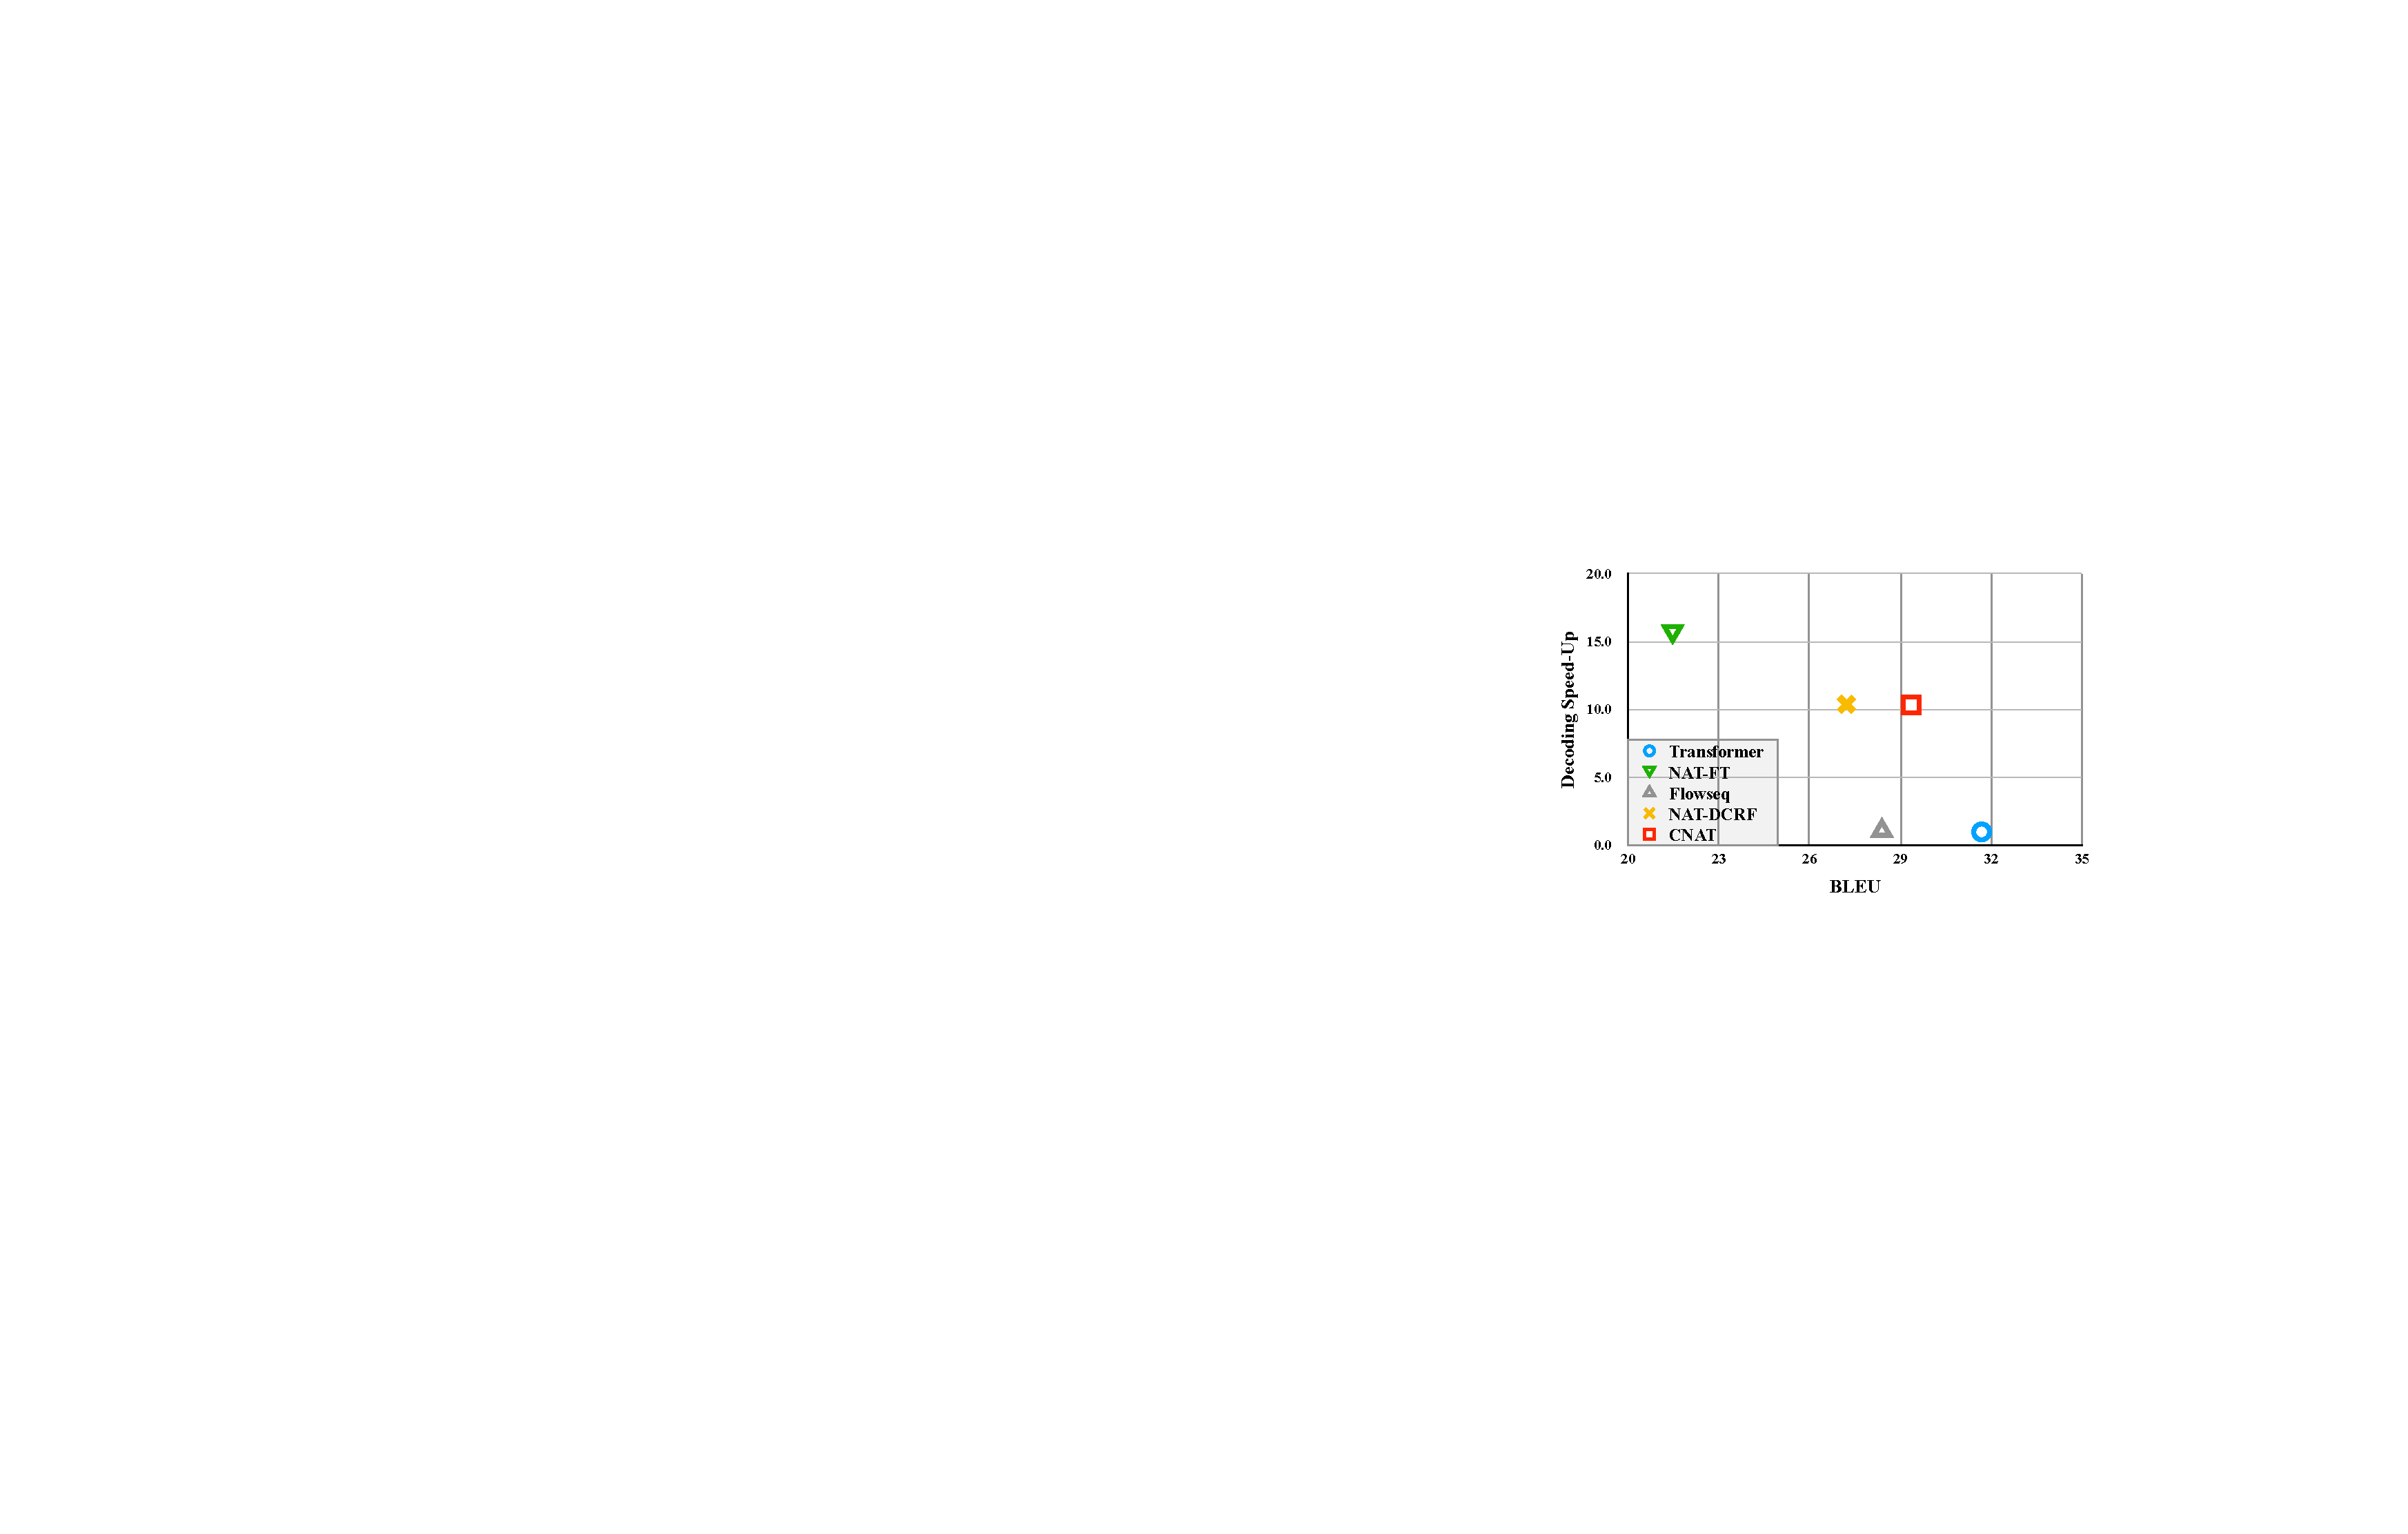
\includegraphics[width=1.0\linewidth]{figures/pure-speed.pdf}
    \caption{Pure NAT decoding.}
    \label{fig:pure_speed}
    \end{subfigure}
    \begin{subfigure}[t]{0.495\linewidth}
    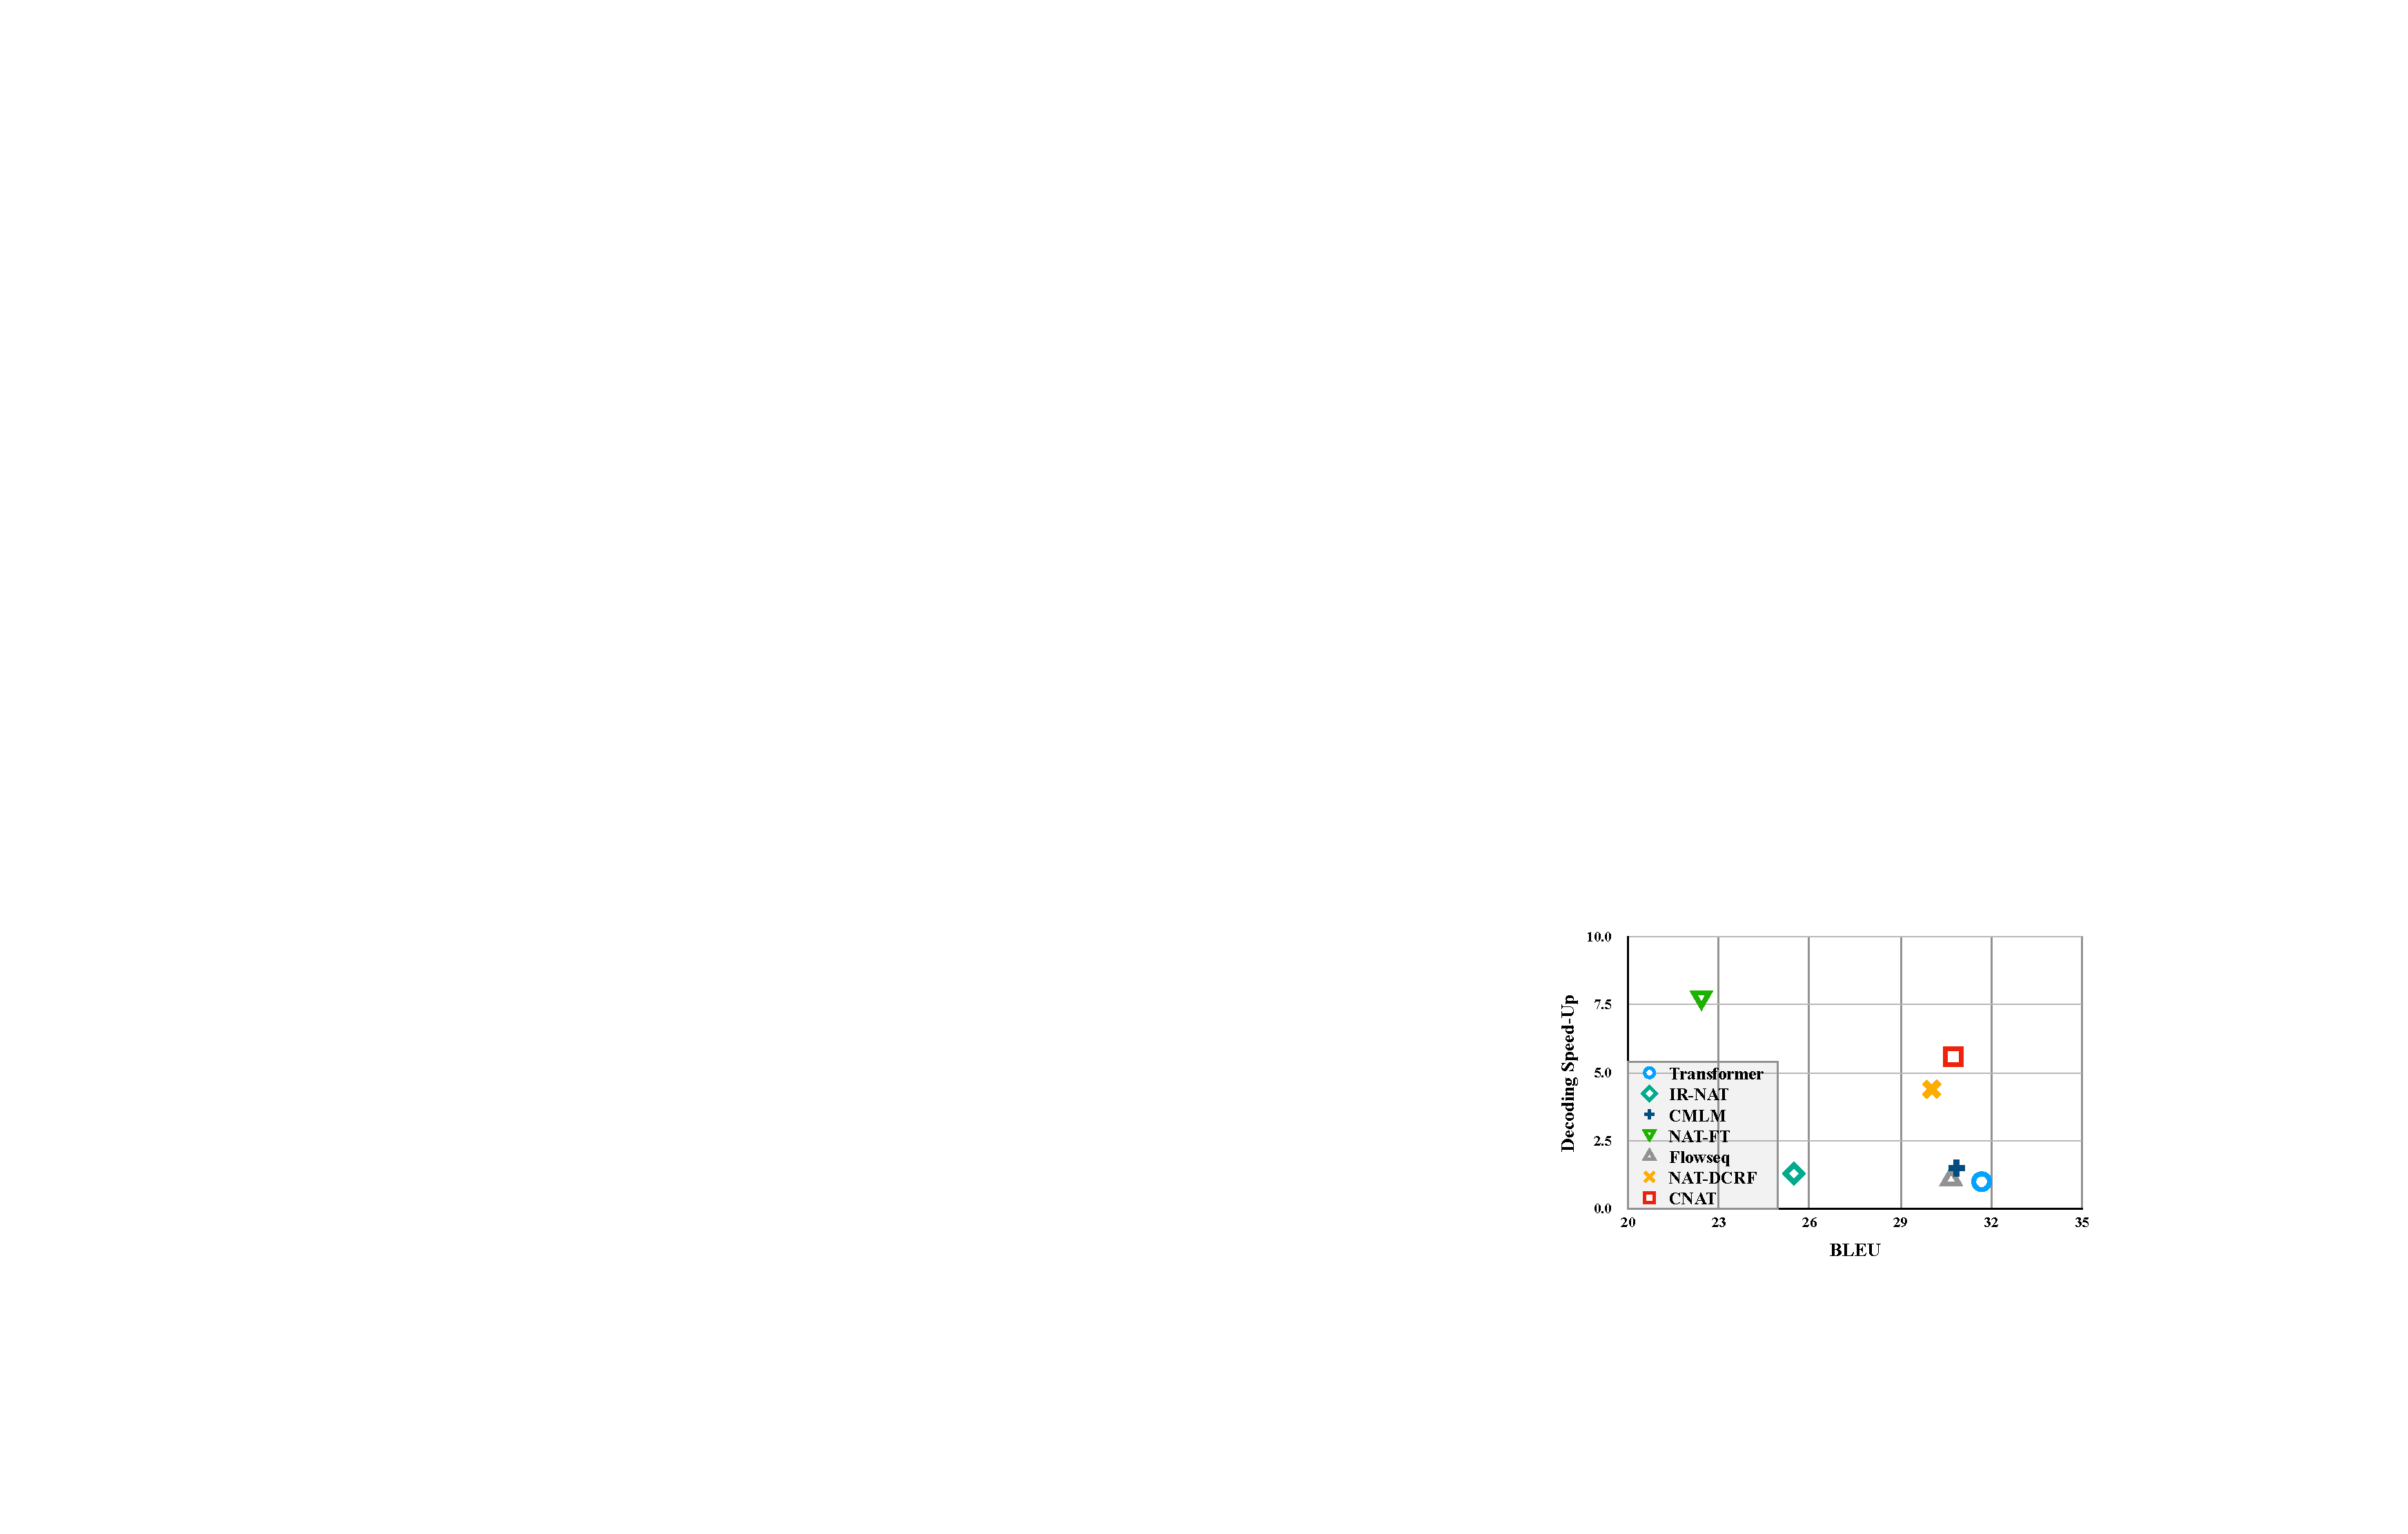
\includegraphics[width=1.0\linewidth]{figures/adv-speed.pdf}
    \caption{NAT with advanced decoding techniques.}
    \centering
    \label{fig:adv_speed}
\end{subfigure}
\caption{BLEU and decoding speed-up of NAT models on WMT14 DE-EN test set. Each point represents the decoding method run with its corresponding setting in Table~\ref{tab:kd_mt}, Table~\ref{tab:lpd_mt} or Table~\ref{tab:iter_mt}. }
\label{fig:speed}
\end{figure*}
\paragraph{Translation Efficiency.} 
As depicted in Figure~\ref{fig:speed}, we validate the efficiency of~\method. 
Put simply, the decoding speed is measured sentence-by-sentence, and the speed-up is computed by comparing it with the Transformer.
Figure~\ref{fig:pure_speed} and Figure~\ref{fig:adv_speed} show the BLEU scores and decoding speed-up of NAT models. 
The former compares the pure NAT models. 
The latter compares NAT model inference with advanced decoding techniques~(parallel reranking or iterative-based decoding)\footnote{Our results are conducted on a single GeForce GTX 1080-TI GPU. Please note that the result in Figure~\ref{fig:pure_speed} and Figure~\ref{fig:adv_speed} may be evaluated under different hardware settings, and it may not be fair to compare them directly.}.  

We can see from Figure~\ref{fig:speed} that the point of \method is located on the top-right of the baselines. 
The \method outperforms our baselines in BLEU if speed-up is held, and in speed-up if BLEU is held, indicating~\method outperforms previous state-of-the-art NAT methods. 
Although iterative models like CMLM achieves competitive BLEU scores, they only maintain minor speed advantages over Transformer. 
In contrast, \method remarkably improves the inference speed while keeping a competitive performance.

\begin{table}[tbp]
\small
\centering
\begin{tabular}{lcc}
\toprule
Methods                 & Latent BLEU   & Translation BLEU \\
\midrule
\method w/ $\z_\text{ref}$ & 100.00        & 59.12            \\
\method w/ $m_\text{ref}$  & 39.72         & 31.59            \\
\method                    & 38.59         & 31.15           \\ 
\bottomrule
\end{tabular}
\caption{Results on the test of IWSLT14 to analyze the effectiveness of categorical modeling. ``w/ $\z_\text{ref}$'' denote \method generate the tokens condition on the latent sequence which is quantized from the reference target. ``w/ $m_\text{ref}$'' denote the~\method generate the tokens condition on the reference length. }
\label{tab:latent_prediction}
\end{table}
\paragraph{Effectiveness of Categorical Modeling.}
We further conduct the experiments on the test set of IWSLT14 to analyze the effectiveness of our categorical modeling and its influence on translation quality. 
We regard the categorical predictor as a sequence-level generation task and list its BLEU score in Table~\ref{tab:latent_prediction}.

As see, a better latent prediction can yield a better translation. 
With the $\z_\text{ref}$ as the latent sequence, the model achieves surprisingly good performance on this task, showing the usefulness of the learned categorical codes. 
We also can see that the~\method decoding with reference length only slightly ~(0.44 BLEU) better than it with predicted length, indicating that the model is robust.

\begin{table}[tbp]
\centering
\tabcolsep 4pt
\small
\begin{tabular}{ccccccccc}
\toprule
\multirow{2}{*}{Line}&\multicolumn{3}{c}{$K$} && \multicolumn{2}{c}{Predictor} &\multirow{2}{*}{GateNet} & \multirow{2}{*}{BLEU}   \\ \cmidrule{2-4} \cmidrule{6-7}
 &32    & 64    & 128   && CRF         & AR              &                          &  \\\midrule
1&\hit  &       &       && \hit        &                 & \hit                     & 30.13    \\
2&      & \hit  &       && \hit        &                 & \hit                     &\textbf{31.87} \\
3&      &       & \hit  && \hit        &                 & \hit                     & 30.82    \\
4&      & \hit  &       && \hit        &                 &                          & 29.32    \\
5&      & \hit  &       &&             & \hit            & \hit                     & 28.23    \\
6&      & \hit  &       &&             & \hit            &                          & 24.00    \\
7&      &       & \hit  &&             & \hit            &                          & 25.43    \\
8&      &       &       &&             &                 &                          & 24.25    \\
\bottomrule
\end{tabular}
\caption{Ablation study on the dev set of IWSLT14. Note that we train all of the configurations with knowledge distillation. ``AR'' denotes an autoregressive Transformer predictor. The line 8 is our NAT baseline.}
\label{tab:ablation}
\end{table}
\subsection{Ablation Study}
We further conduct the ablation study with different \method variant on dev set of IWSLT14. 

\paragraph{Influence of $K$.}
We can see the CRF with the categorical number $K=64$ achieves the highest score~(line 2).  
A smaller or larger $K$ neither has a better result. 
The AR predictor may have a different tendency: with a larger $K=128$, it achieves a better performance. 
However, a larger $K$ may lead to a higher latency while inference, which is not the best for non-autoregressive decoding.
In our experiments, the $K=64$ can achieve the high-performance and be smaller enough to keep the low-latency during inference. 

\paragraph{CRF versus AR.} 
Experiment results show that the CRF-based predictor is better than the AR predictor. 
We can see that the CRF-based predictor surpasses the Transformer predictor 3.5 BLEU (line 2 vs. line 5) with the GateNet;
without the GateNet, the gap enlarges to 5.3 BLEU (line 4 vs. line 6). 
It is consistent with our intuition that CRF is better than Transformer to model the dependencies among latent variables on machine translation when the number of categories is small. 

\paragraph{GateNet.} 
Without the GateNet, the \method with AR predictor degenerates a standard LT model with a smaller latent space. 
We can see its performance is even lower than the NAT-baselines~(line 6 vs. line 8). 
Equipping with the GateNet and the schedule sampling, it outperforms the NAT baseline with a large margin~(around 4.0 BLEU), showing that the GateNet mechanism plays an essential role in our proposed model.

\subsection{Code Study}
To analyze the learned category, we further compute its relation to two off-the-shelf categorical information: the part-of-speech~(POS) tags and the frequency-based clustered classes.
For the former, we intuitively assign the POS tag of a word to its sub-words and compute the POS tag frequency for the latent codes. 
For the latter, we roughly assign the category of a subword according to its frequency.
It needs to mention that the number of frequency-based classes is the same as that of the POS tags.

\begin{table}[tbp]
\small
\tabcolsep 3pt
\centering
\begin{tabular}{lccc} 
\toprule
               & \textbf{H-score}   & \textbf{C-score}  & \textbf{V-measure}    \\
\midrule
w/ POS tags    & \textbf{0.70}      & 0.47              & \textbf{0.56}         \\
w/ Frequency   & 0.62               &\textbf{0.48}      & 0.54                  \\
\bottomrule
\end{tabular}
\caption{Clustering evaluation metrics on the test set of IWSLT14 to analyze the learned codes. }
\label{tab:cluster}
\end{table}
\paragraph{Quantitative Results.} 
We first compute the V-Measure~\cite{vmeasure} score between the latent categories to POS tags and sub-words frequencies. 
The results are listed in Table~\ref{tab:cluster}.

Overall, the ``w/ POS tags'' achieves a higher V-Measure score, indicating that the latent codes are more related to the POS tags than sub-words frequencies.
The homogeneity score (H-score) evaluates the purity of the category.
We also can see that the former has a relatively higher H-score than the latter (0.70 vs. 0.62),  which is consistent with our intuition.

\begin{figure}[tbp]
\centering
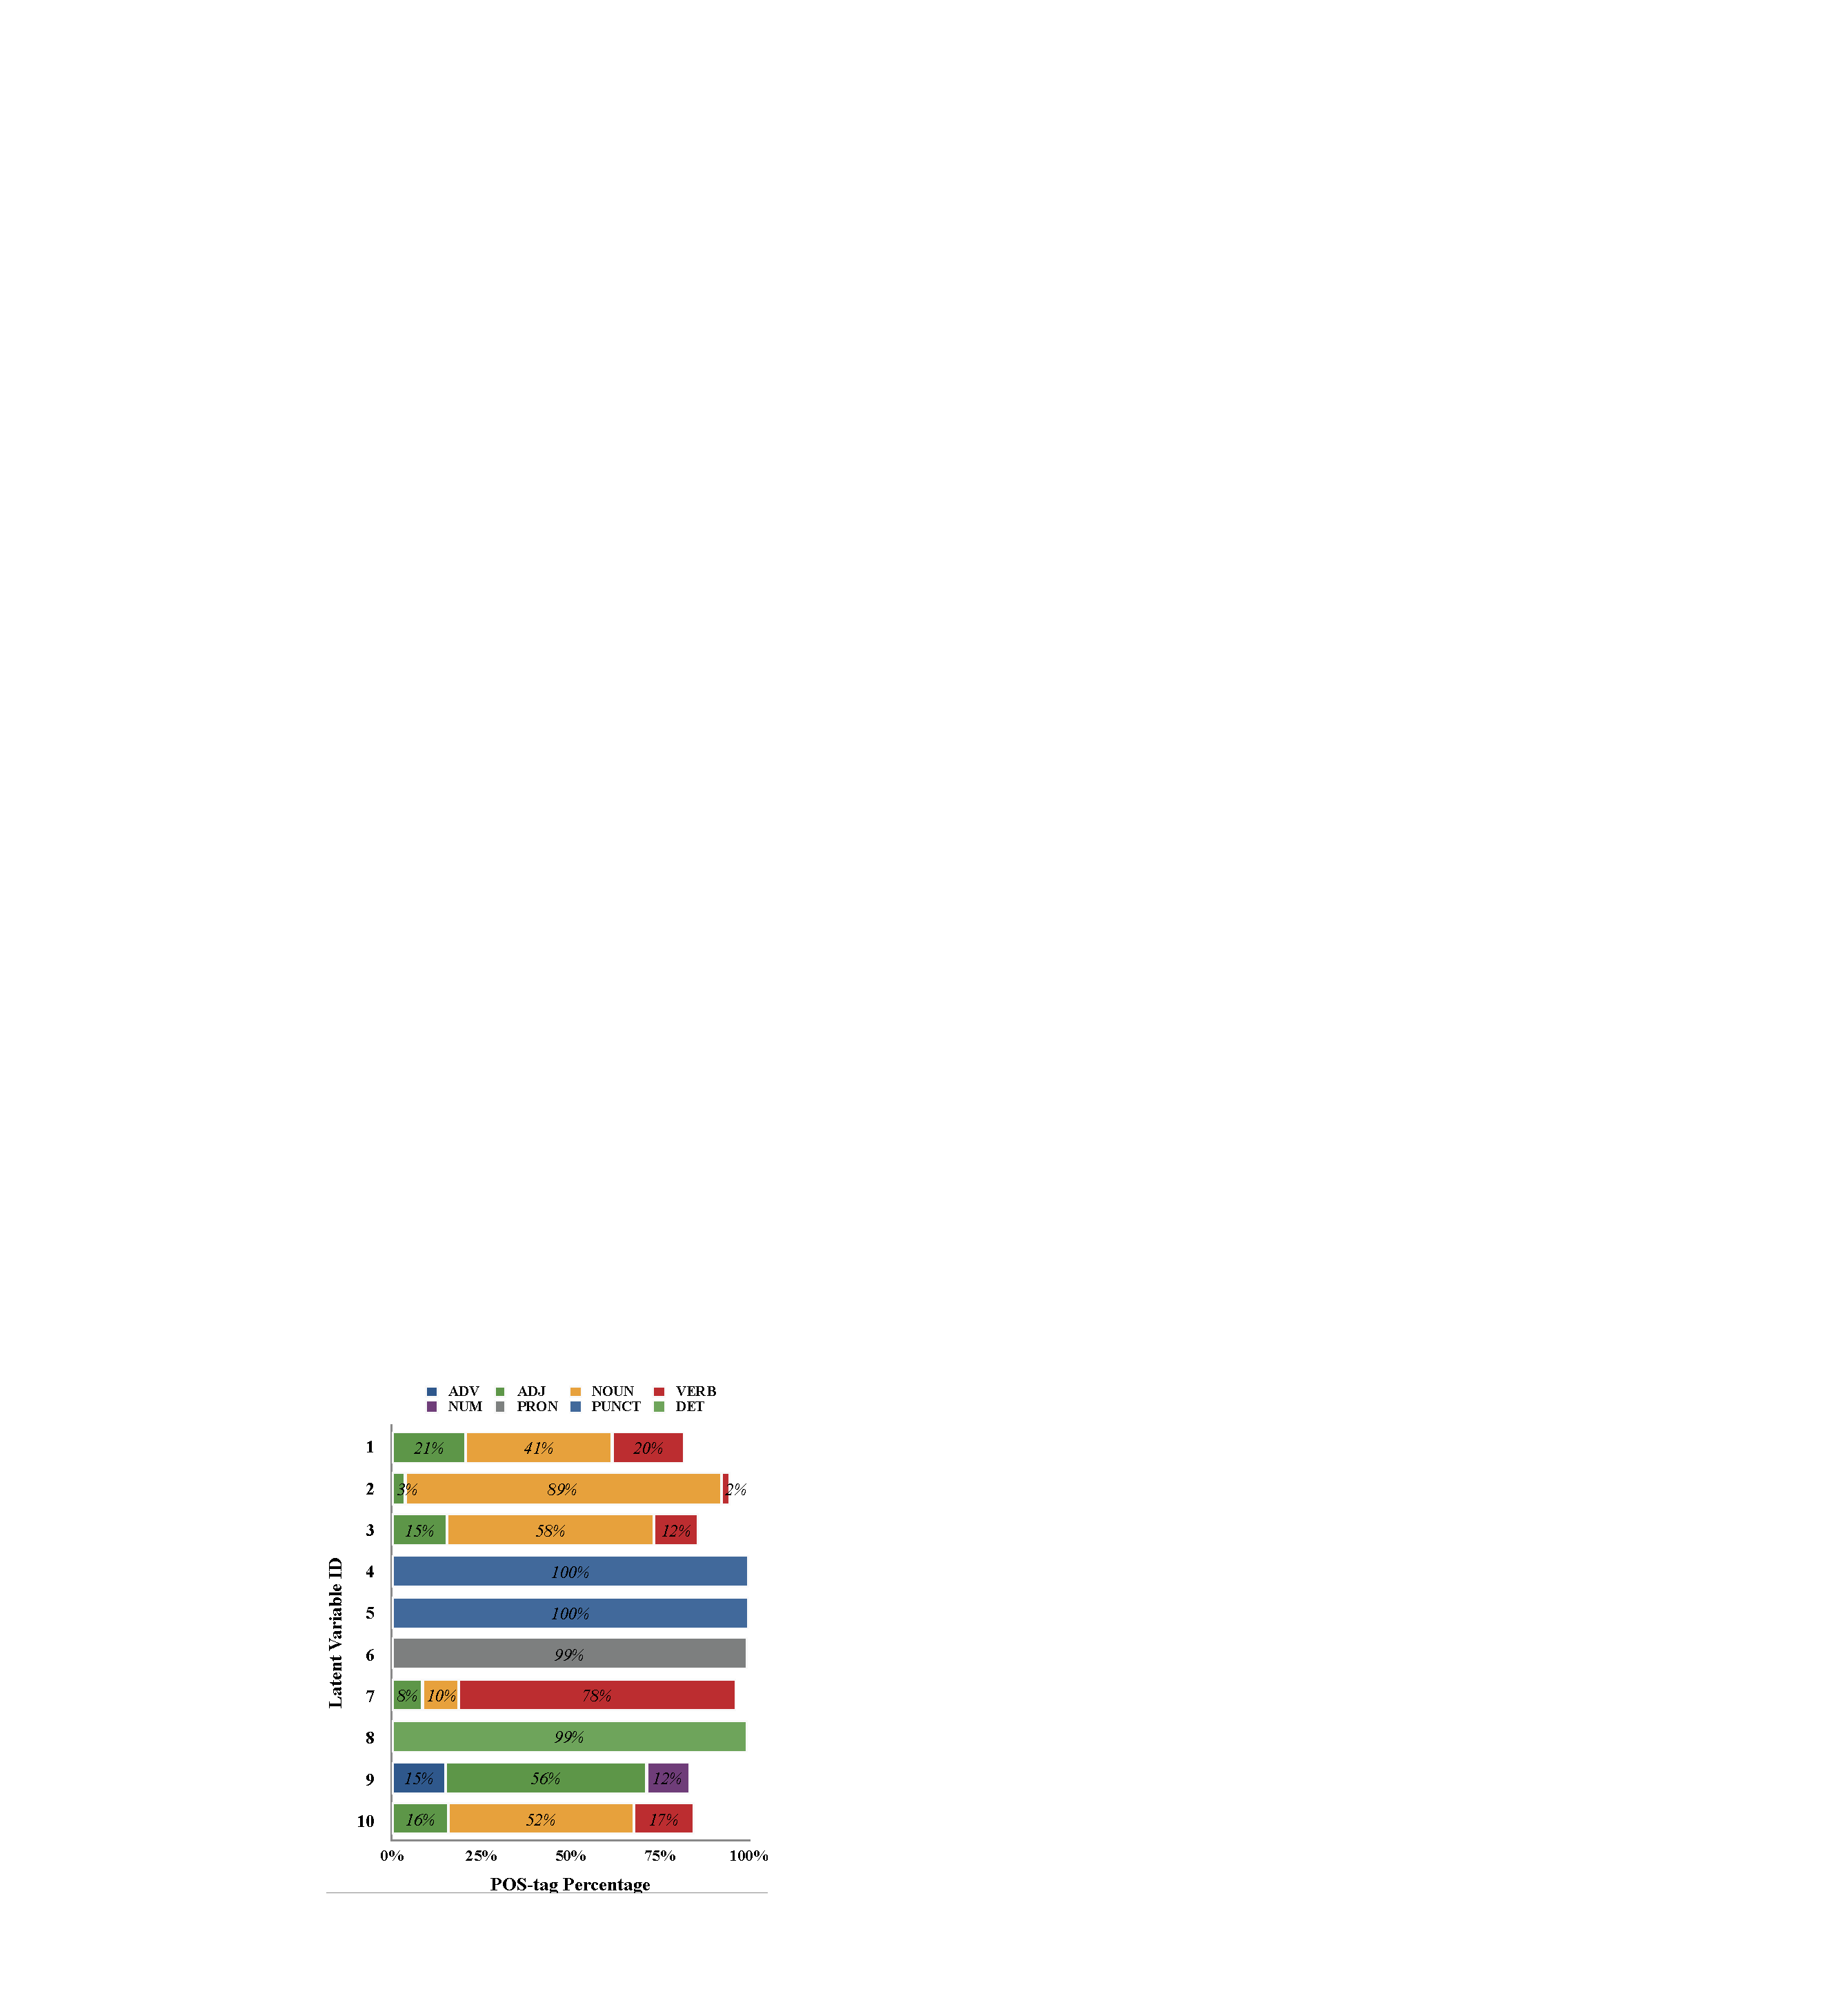
\includegraphics[width=\linewidth]{figures/codes3.pdf}
\caption{The POS tags distribution for the top 10 frequent latent variables on the test set of IWSLT14. We list the top 3 frequent POS tags for each latent variable. }
\label{fig:pos_dist}
\end{figure}
\paragraph{Case Analysis.} 
As shown in Figure~\ref{fig:pos_dist}, we also depict the POS tags distribution for the top 10 frequent latent variables on the test set of IWSLT14\footnote{More details can be found in Appendix B.}. 
We can see a sharp distribution for each latent variable, showing that our learned fuzzy classes are meaningful. 


